\documentclass[letterpaper, 10pt, conference]{ieeeconf}
\IEEEoverridecommandlockouts
\overrideIEEEmargins

\usepackage{amssymb}
\usepackage{amsmath}
% \usepackage{cite}
\usepackage[utf8]{inputenc}
\usepackage{graphicx}
\usepackage{hyperref}
\usepackage{xcolor}
\usepackage{algorithm}
\usepackage{algpseudocode}
\usepackage[sorting=none]{biblatex}
\addbibresource{egbib.bib}

\newcommand{\todo}[1]{\textcolor{red}{\textbf{TODO:} #1}}

\title{\LARGE \bf Analyzing the speed-accuracy tradeoff in human reaching with trajectory optimization and motor noise}
\author{Riley Bridges, Ethan Parham}

\begin{document}

\maketitle
\thispagestyle{plain}
\pagestyle{plain}

\begin{abstract}
\todo{rewrite this} \\
The cause of the speed-accuracy tradeoff is a debated topic of interest in motor neuroscience. Two prominent theories are the presence of signal dependent motor noise and planning variability. In this work, we aim to determine how well the presence of both factors simultaneously explains the speed-accuracy tradeoff. A human arm reaching model is developed with bio-realistic signal dependent motor noise, and a Gaussian noise model is used to deterministically approximate the motor noise. Trajectory optimization is used to simulate several different reaching tasks with varying target sizes and movement durations. These reaching trajectories are then compared to experimental human reaching data as well as experimentally observed trends, revealing a high degree of similarity. These results suggest the speed-accuracy tradeoff is likely caused by a combination of these two factors.
\end{abstract}

\section{Introduction}
\todo{condense this for ACC audience} \\
The speed-accuracy tradeoff is a phenomena in motor neuroscience which describes the relationship between the speed of a motion and the accuracy required of the task being performed. The presence of the speed-accuracy tradeoff means that the more accuracy a movement requires, the more time the movement will take and vice versa. It is easy to observe the phenomena in many activities in daily life. Even tasks as simple as moving a computer mouse to control a cursor clearly demonstrate the increased precision gained from low movement speed. The speed-accuracy tradeoff is fairly ubiquitous across different animal species as well as motor, perceptual, and cognitive tasks \cite{zimmerman_book}. As a result, understanding the relationship is a frequent topic of study, as the tradeoff must be considered in order to produce accurate models of a controlled motion \cite{speed_accuracy_history}, reaction time, and accuracy \cite{hierarchical_speed_accuracy}. The tradeoff can be quantitatively modeled using Fitts’ law. Fitts’ Law relates the width of the target of motion $W$, the movement distance $A$, and the movement duration $MD$, as shown below \cite{fitts_law}. Fitts law is frequently used in combination with empirical data from laboratory testing to determine the efficacy of models in relation to the speed-accuracy tradeoff.  

\begin{equation}
    MD = a + b \log_2 \left(\frac{2A}{W}\right) \label{eq:fitts_law}
\end{equation}

 Historically, the speed-accuracy tradeoff has been attributed to signal dependent motor noise, which is noise which has increasing variance depending on the strength of a neural control signal \cite{signal_dependent_motor_noise}. Noise in neural control will cause a change in the desired trajectory of a motion. These perturbations will eventually result in inaccuracies in the final movement. If noise was not a factor in the control of motion, then theoretically faster movements would result in less motor inaccuracy since there would be less time for noise to make an impact on the motion. In fact, the opposite is true as shown by Fitts’ law. The conclusion therefore is that higher speeds result in larger noise signals in motor control, resulting in larger movement variability.

 However, a new development proposes that a biomechanically realistic computational model can demonstrate the speed-accuracy tradeoff without incorporating motor noise \cite{original_paper_high_fidelity}. The findings propose that the speed-accuracy tradeoff is caused by tighter constraints in trajectory optimization for an accurate problem which reduces the number of fast solutions for the problem. As a result, motor planning variability is the root cause of the speed-accuracy tradeoff and not the motor noise as previously proposed. In order to reach this conclusion, the researchers employed a three dimensional, five degree-of-freedom model of the arm utilizing 47 muscles to produce realistic motions. Then, they utilized minimization of a cost function to model point to point movements in order to synthesize movement. They found that the motor variability can be explained using optimal control theory. Essentially, when a movement is being planned, if there is a large target there are many potential optimal paths which are found using the stochastic optimizer. Since there are more potential solutions to the movement problem, there will be many “good” solutions. However, if the search space is decreased by increasing the required accuracy needed for the movement, there will be fewer “good” options, and a less efficient option is more likely to be found when compared to a movement with lower required accuracy. 
 \par Their hypothesis about motor planning was further reinforced using a study of the motor cortex of a Rhesus monkey by correlating data for the preparatory neural state variability for accurate and inaccurate tasks to the movement variability. This further emphasizes that motor planning variability results in variability in the executed motion, and indicates some kind of optimal control is involved in motor planning.

A key emphasis of the researchers is the further room for improvement on their model. Signal dependent noise and motor planning optimization are likely both contributors to the speed-accuracy tradeoff as they both are able to correlate to Fitts’ law, so a model which combines both would be an improvement over either model on its own. Additionally, improvement on the optimizer used would also have potential to increase the accuracy of the model \cite{deep_rl}.

The methods humans and animals use to optimize their motions is of great interest beyond just better modeling the reaching of a human arm. Humans are capable of performing and optimizing very complex tasks, which is a capability which is highly desirable in robotics \cite{biometric_human_arm}. Better understanding the speed-accuracy tradeoff and the methods which are used to reduce redundancy in motion will help further the abilities of robots to perform difficult and complex tasks.

\todo{adapt this into related work section} \\
The decision to combine noise into a trajectory optimization model meant we needed to find more information on modeling signal dependent noise. This led to the frequently referenced model by Harris and Wolpert \cite{signal_dependent_motor_noise}. This model applied white noise to the neural command signal that activates muscles. The noise is increased proportionally to the control signal strength. In order to add noise into a trajectory optimization model, we began researching other potential models which combined both noise and trajectory optimization. This lead us to the model by Todorov and Li \cite{ilqg}, which uses an iterative LQG model for locally-optimal feedback control which incorporates control dependent noise. Todorov found the control dependent noise has a similar effect to an energy cost, and utilized a stochastic model of the human arm with six muscle actuators in their model. Their work was further iterated on by Van Wouwe et al. \cite{stochastic_model}, who determined that the iLQG model required assumptions and tuning which might not be physically realistic. They acknowledged that the hand tuned cost functions were a simplifaction that potentially sacrificed accuracy. As a result, the Van Wouwe model uses stochastic simulations for both feedforward and feedback control their nonlinear musculoskeletal model, which also uses six muscles. 

We immediately recognized the potential usefulness of this model, as it was implemented in MATLAB and was freely available on github. As a result, when we decided to transition away from using the complex 47 muscle model, it was a clear choice to make. The model already included a framework for modeling reaching trajectories in the presence of both signal and motor noise, and although it was not geared towards analyzing the speed-accuracy tradeoff it would not be overly difficult to adapt it for that purpose. We also considered using the model proposed by Peternel, et al. \cite{cost_benefit_tradeoff}, which also examined stochastic optimization in the presence of motor noise, while also focusing on the speed-accuracy tradeoff. However, this model was not readily avaliable to download, so we decided against attempting to recreate it in favor of adapting the Van Wouwe model.

\section{Problem Formulation}

We aimed to answer the following questions: 
\begin{itemize}
    \item When using trajectory optimization to simulate reaching movements on a human arm model, how well does the simulated behavior match human behavior, particularly with respect to the speed-accuracy tradeoff? (Question studied in \cite{original_paper_high_fidelity})

    \item How does the introduction of signal-dependent motor noise to the model affect this comparison?

    \item How does this behavior change when simulating execution of reaching movements using feedback control rather than just planning them?
    % \item How does the use of different trajectory optimization methods affect this comparison?
\end{itemize}
For each of these questions, we used the following metrics to compare the simulated behavior (collected from our models) to human behavior (experimental data collected and used in \cite{original_paper_high_fidelity}):
\begin{itemize}
    \item Similarity of hand velocity profile during center-out fast reaching movements, evaluated qualitatively by appearance and quantitatively by time and value of maximum velocity:
    \begin{align}
        V_{\text{max}} &= \max \left|V_{\text{sim}}(t)\right| \\
        T_{\text{max}} &= \arg\max_{t \in [0, t_f]} \left|V_{\text{sim}}(t)\right|
        % \delta_{V_{\text{max}}} &= \max \left|V_{\text{sim}}(t)\right| - \max \left|V_{\text{exp}}(t)\right| \\
        % \delta_{T_{\text{max}}} &= \arg\max_{t \in [0, t_f]} \left|V_{\text{sim}}(t)\right| - \arg\max_{t \in [0, t_f]} \left|V_{\text{exp}}(t)\right|
    \end{align}
    Where $V_{\text{sim}}$ is the simulated velocity of the hand during its reaching trajectory, and $t_f$ is the time at which the hand reaches the target.
    % , $V_{\text{exp}}$ is the experimentally measured velocity of the hand during its reaching trajectory,

    \item Delay in time of maximum velocity between large and small targets:
    \begin{multline}
        t_{\text{delay}} = \arg\max_{t \in [0, t_f]} \left|V_{\text{sim}}^{L}(t)\right| - \arg\max_{t \in [0, t_f]} \left|V_{\text{sim}}^{S}(t)\right|
        % - \left(\arg\max_{t \in [0, t_f]} \left|V_{\text{exp}}^{L}(t)\right| - \arg\max_{t \in [0, $V_{\text{exp}}$ is the experimentally measured velocity of the hand during its reaching trajectory,, t_f]} \left|V_{\text{exp}}^{S}(t)\right|\right)
    \end{multline}
    Where $V_{\text{sim}}^{L}$ and $V_{\text{sim}}^{S}$ are the simulated velocities of the hand during its reaching trajectory to large and small targets, respectively.
    % $V_{\text{exp}}^{\text{large}}$ and $V_{\text{exp}}^{\text{small}}$ are defined similarly.
    \item Fitts' Law model parameters $a$ and $b$.
    Several reaching tasks with variable target distance and target width will be simulated. A least squares regression will then be performed on the resulting movement duration data from each trial in order to fit the parameters:
    \begin{align}
        \begin{bmatrix}
            a^* \\ b^*
        \end{bmatrix} &= \arg\min_{a, b} \sum_{i=1}^N \left(MD_i - \left(a + b \log_2\left(\frac{2A_i}{W_i}\right)\right)\right)^2
    \end{align}
    Where $MD_i$ is the movement duration, $A_i$ the target distance, and $W_i$ the target width for the $i$th trial, and $N$ is the number of trials.
\end{itemize}

\subsection{System Model and Dynamics}
We model the human arm as a two degree of freedom planar arm with shoulder and elbow joints, actuated by six Hill-type muscles. This model has been adapted from the model used in \cite{stochastic_model}, and a diagram of the model is shown in figure \ref{fig:arm_model}. 

\begin{figure}[h]
    \centering
    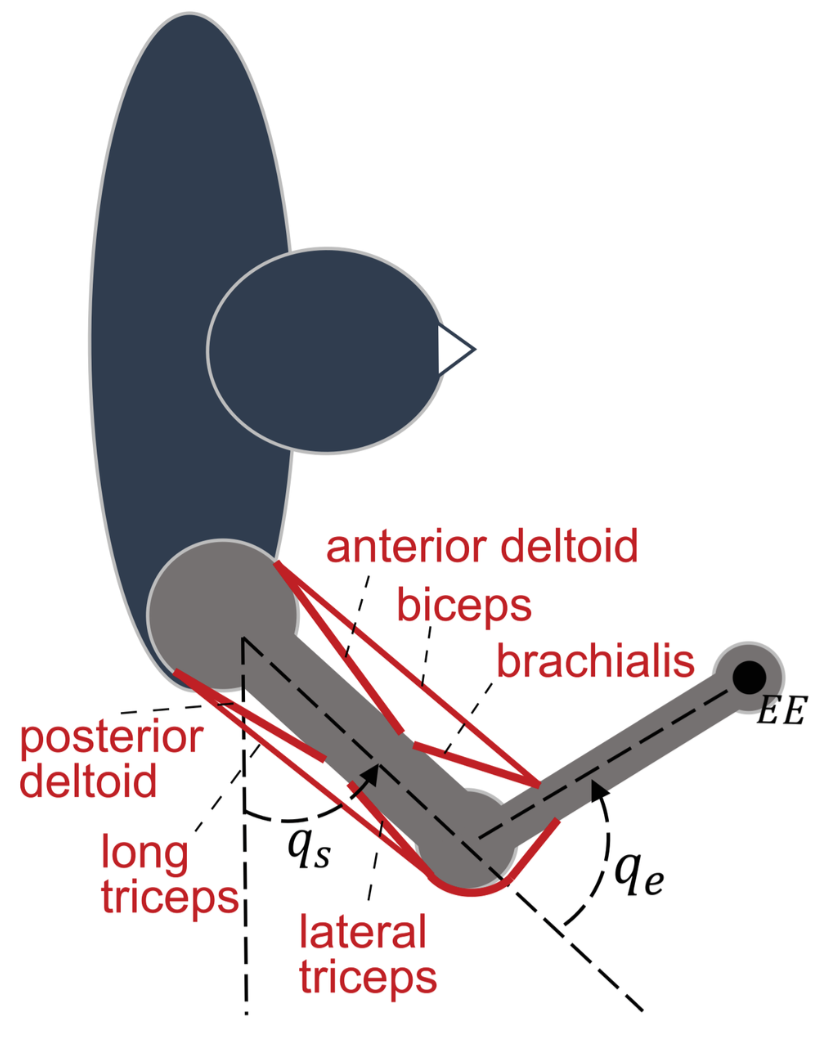
\includegraphics[width=0.3\textwidth]{images/arm_model_diagram.png}
    \caption{Diagram of the musculoskeletal human arm model \cite{stochastic_model}.}
    \label{fig:arm_model}
\end{figure}

The state and control input vectors are defined below:
\begin{align}
    \mathbf{x} &= \begin{bmatrix}
        \mathbf{q} &
        \dot{\mathbf{q}}
    \end{bmatrix}^\top = \begin{bmatrix}
        \theta_s &
        \theta_e &
        \dot{\theta}_s &
        \dot{\theta}_e
    \end{bmatrix}^\top \\
    \mathbf{u} &= \begin{bmatrix}
        a_{\text{brach}} & a_{\text{lattri}} & a_{\text{antdel}} & a_{\text{postdel}} & a_{\text{bic}} & a_{\text{lattri}}
    \end{bmatrix}
\end{align}

Where $\theta_s$ and $\theta_e$ are the shoulder and elbow joint angles, respectively, and $\dot{\theta}_s$ and $\dot{\theta}_e$ are the corresponding joint angular velocities. The control input $\mathbf{u}$ is a vector of muscle activations for each of the 6 muscles in the model. The stochastic dynamics of the system are given by the following differential equation:
\begin{align}
    \dot{\mathbf{x}} &= f(\mathbf{x}, \mathbf{u}, \mathbf{w}) \quad \mathbf{w} \sim \mathcal{N}(0, \Sigma_w) \\
    &= \begin{bmatrix}
        \dot{\mathbf{q}} \\
        M(\mathbf{q})^{-1} \left(C(\mathbf{q}, \dot{\mathbf{q}}) + T_M(\tilde{\mathbf{u}}, \mathbf{q})\right)
    \end{bmatrix} \\
    \tilde{\mathbf{u}} &= \mathbf{u} + \text{diag}(\mathbf{u}) \cdot \mathbf{w}
\end{align}
Where $M(\mathbf{q})$ is the mass matrix of the arm model, $C(\mathbf{q}, \dot{\mathbf{q}})$ is the term describing the Coriolis forces, and $T_M(\mathbf{u}, \mathbf{q})$ is the term describing the torques generated by the muscles. Further details on the muscle dynamics of the system can be found in \cite{stochastic_model}. Note that the noise vector is effectively scaled element-wise by the control input vector, thus modeling signal dependent motor noise as described earlier.

Following the work of \cite{stochastic_model}, we approximate the stochastic state trajectories of the system as normally distributed trajectories. This allows us to represent the stochastic state trajectory as a mean trajectory $\mathbf{\bar{x}}(t)$ and a covariance trajectory $P(t)$. We can then use this representation to create a deterministic first order approximation of the dynamics: 
\begin{align*}
    \mathbf{\dot{\bar{x}}}(t) &= f(\mathbf{\bar{x}}(t), \mathbf{u}(t), 0) \\
    \dot{P}(t) &= A(t)P(t) + P(t)A(t)^\top + C(t) \Sigma_w C(t)^\top \\
    &\quad A(t) = \frac{\partial f}{\partial \mathbf{x}}\bigg|_{\mathbf{\bar{x}}(t), \mathbf{u}(t), 0} \\
    &\quad C(t) = \frac{\partial f}{\partial \mathbf{w}}\bigg|_{\mathbf{\bar{x}}(t), \mathbf{u}(t), 0}
\end{align*}

\subsection{Trajectory Optimization}
\todo{Make this more general to account for MPC and separate it from approach/methods section} \\
To plan the trajectory of the arm during a reaching task, we aimed to solve the following optimal control problem:
\todo{add joint bounds and positive time constraint} \\
\begin{align}
    \mathbf{u}^* = \arg\min_{\mathbf{u}(t)} &\quad k_u \cdot \int_0^{t_f} \mathbf{u}(t)^\top R \mathbf{u}(t) dt + k_t \cdot t_f \label{eq:cost} \\
    \text{subject to} &\quad \mathbf{\dot{\bar{x}}}(t) = f(\mathbf{\bar{x}}(t), \mathbf{u}(t), 0), \quad \mathbf{\bar{x}}(0) = \mathbf{x}_0 \label{eq:dynamics_constraint} \\
    \begin{split}
    &\quad \dot{P}(t) = A(t)P(t) + P(t)A(t)^\top \\
    &\quad \quad + C(t) \Sigma_w C(t)^\top, \quad P(0) = P_0 
    \end{split}\label{eq:dynamics_constraint_p} \\
    &\quad \mathbf{\dot{\bar{x}}}(0) = 0, \quad \mathbf{\dot{\bar{x}}}(t_f) = 0 \label{eq:boundary_constraints} \\
    &\quad F_k(\mathbf{\bar{x}}(t_f)) = \mathbf{p}_{\text{target}} \label{eq:target_constraint} \\
    \begin{split}
    &\quad [HP(t_f)H^\top]_{i,i} \leq \sigma_{\text{target}, i}^2 \ , \\
    &\quad H = \frac{\partial F_k}{\partial \mathbf{x}}\bigg|_{\mathbf{\bar{x}}(t_f)}, \quad i = 1, \ldots, n 
    \end{split}\label{eq:target_variance_constraint}
\end{align}

Where $t_f$ is the duration of the trajectory, $R$ is a weight matrix for muscle activations, $k_u$ is a weight for muscle activation, $k_t$ is a weight for duration, $\mathbf{x}_0$ is the initial state of the arm, $P_0$ is the initial state covariance, $F_k$ is the arm forward kinematics function, $\mathbf{p}_{\text{target}}$ is the position of the target, and $\sigma_{\text{target}, i}$ is the desired standard deviation of the final position of the $i$th dimension of the target.

Equation \ref{eq:cost} works to minimize muscle activations and trajectory duration. Equations \ref{eq:dynamics_constraint} and \ref{eq:dynamics_constraint_p} enforce the dynamics of the system. Equation \ref{eq:boundary_constraints} enforces zero velocity and acceleration at the beginning and end of the trajectory, while equation \ref{eq:target_constraint} enforces the final mean position of the arm's end effector to be at the target. Finally, equation \ref{eq:target_variance_constraint} enforces the final position of the arm's end effector to be within a certain standard deviation of the target position. This standard deviation can be adjusted to model variation in target size in order to test the speed-accuracy tradeoff.

% \subsection{Model Selection and Adaptation}
% We initially invested a significant amount of time into adapting the complex 47 muscle OpenSim model for use in our project. However, this model and its supporting trajectory optimization code was developed using a heavily outdated version of OpenSim that is no longer well supported. An attempt was made to transition the model and supporting code to the latest version of OpenSim by adapting to the latest API, but this proved extremely time consuming and difficult to debug due to the complexity of the OpenSim library. As a result, we decided to abandon this model in favor of a simpler model.

% Initially, a more complex human arm model was chosen due to the increased accuracy of the model. This model, used in \cite{original_paper_high_fidelity}, was a biologically accurate musculoskeletal model with 47 Hill-type muscle actuators. However, this model was abandoned due to its use of outdated software (OpenSim version 3.3), difficulty in setting up the development environment, poor cross-platform support, and requiring simulation/control code to be written in C++.

% \subsection{Modeling Signal Dependent Motor Noise}

\section{Approach}

\subsection{Feedforward Planning using Direct Collocation}
\todo{Add citation for direct collocation} \\
Working with the Van Wouwe model, we adapted the optimal control framework from \cite{stochastic_model} to perform only feed forward control and to fit our trajectory optimization problem. This implementation required us to discretize the muscle activation trajectory into a vector of $N$ nodes, and to optimize over that vector. To enforce the dynamics efficiently, we use a method referred to as direct collocation. This involves similarly discretizing the state trajectory into a series of $N$ nodes that are added to the design vector, and then enforcing the dynamics constraints between each consecutive node. This formulation results in the following design vector:

\begin{align}
    \mathcal{X} &= \begin{bmatrix}
        \mathbf{u}_1  \cdots \mathbf{u}_N & \mathbf{\bar{x}}_1 \cdots \mathbf{\bar{x}}_N & P_1 \cdots P_N & t_f
    \end{bmatrix}^\top
\end{align}

Where $\mathbf{u}_i$, $\mathbf{\bar{x}}_i$, and $P_i$ are the muscle activations, state, and state covariance at the $i$th node, respectively. Then the discretized optimization problem can be formulated as follows:
\todo{change to actual fancier discretization used or at least mention it as a note} \\

\begin{align}
    \mathbf{u}^* = \arg\min_{\mathbf{u}} &\quad k_u \cdot \sum_{i=1}^{N} \mathbf{u}_i^\top R \mathbf{u}_i + k_t \cdot t_f \label{eq:dcost} \\
    \text{subject to} &\quad \mathbf{\bar{x}}_{i+1} = \mathbf{\bar{x}}_i + f(\mathbf{\bar{x}}_i, \mathbf{u}_i, 0) \delta t \\
    \begin{split}
        &\quad P_{i+1} = (I + A_i \delta t)P_i(I + A_i \delta t)^\top \\
        &\quad \quad + C_i \Sigma_w C_i^\top \delta t
    \end{split} \label{test} \\
    &\quad \mathbf{\bar{x}}_1 = \mathbf{x}_0, \quad f(\mathbf{\bar{x}}_0, \mathbf{u}_0, 0) = 0 \\
    &\quad f(\mathbf{\bar{x}}_N, \mathbf{u}_N, 0) = 0, \quad F_k(\mathbf{\bar{x}}_N) = \mathbf{p}_{\text{target}} \label{eq:dtarget_constraint} \\
    &\quad [HP_NH^\top]_{i,i} \leq \sigma_{\text{target}, i}^2, \quad H = \frac{\partial F_k}{\partial \mathbf{x}}\bigg|_{\mathbf{\bar{x}}_N} \\
    &\quad i = 1, \ldots, n \label{eq:dtarget_variance_constraint}
\end{align}

Note at the dynamics of the mean and covariance trajectories are enforced using simple forward Euler integration. We may experiment with different integration methods in the future to improve accuracy.

\subsection{Model Predictive Feedback Control}
To simulate the act of executing a reaching motion, rather than just planning it, we implemented a nonlinear model predictive controller (MPC). This controller uses the same nonlinear trajectory optimization problem as the feedforward planner, and simply solves that problem at each iteration of the controller. The control algorithm is detailed in Algorithm \ref{alg:mpc}.

\begin{algorithm}
\caption{Model Predictive Feedback Simulation}\label{alg:mpc}
 \hspace*{\algorithmicindent} \textbf{Input} \\
%  \textbf{Input} \\
    \hspace*{\algorithmicindent} \quad $\mathbf{x}_0$: initial arm state \\
    \hspace*{\algorithmicindent} \quad $t_{\text{iter}}$: duration to execute before replanning \\
    \hspace*{\algorithmicindent} \quad $\mathbf{p}_{\text{target}}$: target position \\
    \hspace*{\algorithmicindent} \quad $\sigma_{\text{target}}$: target standard deviation \\
    \hspace*{\algorithmicindent} \quad $N$: number of nodes in trajectory 
\begin{algorithmic}
\State $\mathbf{x}_{\text{current}} \gets \mathbf{x}_0$
\While{$\|F_k(\mathbf{x}_{\text{current}}) - \mathbf{p}_{\text{target}}\| > \sigma_{\text{target}}$}
    \State $\mathbf{u}^*, \delta t \gets \text{SolveOptimization}(\mathbf{x}_{\text{current}}, \mathbf{p}_{\text{target}}, \sigma_{\text{target}}, N)$
    \State $N_{\text{iter}} \gets \min(\lceil t_{\text{iter}} / \delta t \rceil, N)$
    \For{$i = 1$ to $N_{\text{iter}}$}
        \State $\mathbf{w} \gets \mathcal{N}(0, \Sigma_w)$
        \State $\mathbf{x}_{\text{current}} \gets \mathbf{x}_{\text{current}} + f(\mathbf{x}_{\text{current}}, \mathbf{u}_i^*, \mathbf{w}) \delta t$
    \EndFor
\EndWhile
\end{algorithmic}
\end{algorithm}

\subsection{Implementation}
To execute both our feedforward planning and feedback MPC simulations, the algorithms were implemented in MATLAB. 
We used the CasADi library \cite{casadi} as an optimization framework to specify the problem and provide automatic differentiation for gradient and Jacobian computation. The IPOPT nonlinear solver was then used to perform the numerical optimization, with trivial constants provided as initial guesses for elements of the design vector. 
IPOPT was run for a maximum of 3000 iterations, after which the problem was considered infeasible. For MPC simulation, the optimization at the first iteration was solved as described previously, and all consecutive iterations were "warm started" by setting the initial design vector guess equal to the solution from the previous iteration. Most optimization runs converged in less than 500 iterations and took less than 30 seconds to run on a high end consumer grade CPU, although MPC optimization runs that were "warm started" typically converged significantly faster and in fewer iterations. All of the code used to implement the optimization problem can be found in the project GitHub repository: \href{https://github.com/rbridges12/eecs-598-project}{https://github.com/rbridges12/eecs-598-project}. \todo{rename github repo to paper name}

\section{Simulations}
\subsection{Model Validation}

To tune and validate our feedforward planning model, we first performed a series of reaching simulations with different combinations of $k_u$, $k_t$, $\mathbf{x}_0$, $\mathbf{p}_{\text{target}}$, and $\sigma_{\text{target}}$. Target width $W$ was encoded as $\sigma_{\text{target}}$, effectively defining the target as the 95\% confidence ellipse for final end effector position. For each simulation, we recorded the reaching duration and the value and time of the maximum velocity of the end effector mean trajectory. These values were then compared to experimental data from \cite{fitts_law_exp_data} and ideal parameters were chosen based on similarity to the data. The same procedure was followed for the feedback MPC model, except that the actual end effector trajectory was recorded and each trial was repeated several times and averaged to reduce the effect of noise.
Normalized velocity profiles for a slow and a fast trial of the feedforward model are shown in Figure \ref{fig:VelocityFeedforward}, and the same is shown for the feedback MPC model in Figure \ref{fig:VelocityMPC}.

% To determine the prominent kinematic features of our model, we ran reaching simulations across a range of speeds in order to obtain a velocity profile of the simulation. End effector final positions, target radii, and weights for the control effort and duration were selected in order to simulate reaching tasks of various speeds. By increasing the weight of the duration, our simulation optimized for lower movement duration time and as a result the end effector velocity was increased. Increasing the control effort weight demonstrated an opposite effect. Multiple simulations were performed per set of simulation parameters to obtain an average of the end effector velocity across the span of the experiment. Then, both the time and velocity were normalized to have a maximum value of 1 in order to allow comparison between parameter sets. A slow test (movement duration = 0.62s) is shown in Figure \ref{fig:VelocitySlow}, and a fast test (movement duration = 0.28s) is shown in Figure \ref{fig:VelocityFast}. 

\begin{figure}[h]
    \centering
    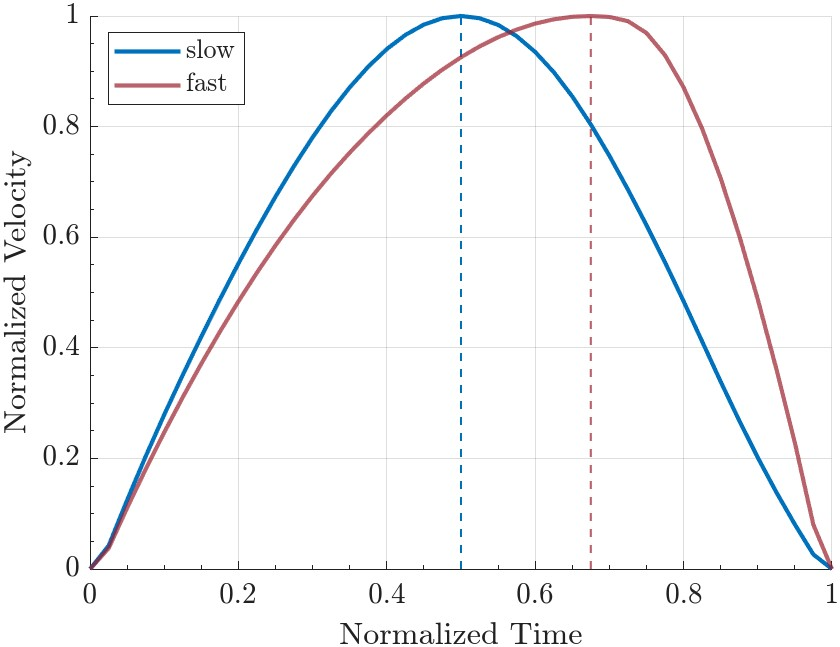
\includegraphics[width=1\linewidth]{images/single_slow_fast.jpg}
    \caption{Normalized end effector velocity profiles for slow and fast feedforward reaching simulations. Each velocity peak is marked with a dashed line.}
    \label{fig:VelocityFeedforward}
\end{figure}

\begin{figure}[h]
    \centering
    \includegraphics[width=1\linewidth]{images/mpc_slow_fast.jpg}
    \caption{Normalized end effector velocity profiles for slow and fast MPC reaching simulations. Profiles of each trial are shown along with the average velocity peaks.}
    \label{fig:VelocityMPC}
\end{figure}
% \begin{table}[]
% \begin{tabular}{|l|l|l|l|l|l|l|}
% \hline
%  & Max Velocity & Time of Max Vel & Distance & Target Radius & $k_u$ & $k_t$ \\ \hline
%  &  &  &  &  &  &  \\ \hline
%  &  &  &  &  &  &  \\ \hline
%  &  &  &  &  &  &  \\ \hline
%  &  &  &  &  &  &  \\ \hline
% \end{tabular}
% \end{table}
% For the feedforward model, the maximum velocity of the slow simulation was 0.76 m/s and occurred at a normalized time of 0.50.

\todo{table of parameters?} \\
% As described in the problem description several metrics were evaluated using the simulated velocity profile data. 
For the fast feedforward trajectory, the maximum velocity was 1.05 m/s and occurred at a normalized time of 0.68. This falls within the range of maximal speeds reported in \cite{soechting_target_size} (0.65-1.35 m/s), and is similar to the simulated maximum velocity from \cite{original_paper_high_fidelity} (1.10 m/s). The control effort weight was 1 and the duration weight was 20, with a movement distance of 0.17 m and a target radius of 0.1 m. For the feedforward slow trajectory, the maximum velocity was 0.76 m/s and occurred at a normalized time of 0.50. The control effort and duration weights were both 1, with a movement distance of 0.27 m and a target radius of 0.05 m. 
When comparing maximum velocities between large and small targets, our model shows a normalized time delay of 0.18 between the two, which is larger but still within the same order of magnitude as the average delay from \cite{soechting_target_size} ($\approx 0.08$). 

The MPC model showed similar results, with the maximum velocity of the fast trajectory falling near the experimental range (2.04 m/s), and occurring at a normalized time of 0.67. The control effort weight was 1 and the duration weight was 100, with a movement distance of 0.36 m and a target radius of 0.1 m. For the slow trajectory, the maximum velocity was 0.76 m/s and occurred at a normalized time of 0.50. The control effort and duration weights were both 1, with a movement distance of 0.27 m and a target radius of 0.05 m. 
The normalized time delay between large and small targets was 0.17, which is similar to the feedforward model.

Qualitatively, these velocity profiles reproduce several trends found in experimental data.
Existing studies show that normalized velocity profiles will be symmetric for medium velocities, shift to the left for slow movements, and shift to the right for fast movements \cite{asymmetric_vel_acc}\cite{human_vel_curves}. 
Our simulations produce a similar trend, with the normalized velocity profile becoming less symmetric as movement duration decreases.
these results are more realistic than a pure motor noise model, which displays primarily symmetric velocity profiles \cite{signal_dependent_motor_noise}; they are also more realistic than a torque model, which shows poorer correlation with experimental data \cite{original_paper_high_fidelity}.
Although the model fails to replicate a shift of the normalized velocity peak to the left at the lowest speed ranges, it importantly replicates the trend of slower movements having earlier peak velocities, which is a key feature of the experimental data.
From these results we can conclude that although our underlying dynamical model is not as accurate as the high fidelity model used in \cite{original_paper_high_fidelity}, both the feedforward and feedback reaching models show a level of realism that make them useful for studying the speed-accuracy tradeoff in reaching movements.

% Quantitatively, these velocity profiles match experimental data quite well. The maximum velocity of the fast feedforward trajectory falls within the range of maximal speeds reported in \cite{soechting_target_size} (0.65-1.35 m/s), and is similar to the simulated maximum velocity from \cite{original_paper_high_fidelity} (1.10 m/s). 
% When comparing maximum velocities between large and small targets, our model shows a normalized time delay of 0.17 between the two, which appears larger but still within the same order of magnitude as the average delay from \cite{soechting_target_size} ($\approx 0.08$). Importantly, the trend of slower movements having earlier peak velocities is present in our model, which is a key feature of the experimental data.

% These velocity profiles display trends present in experimental data, indicating the model reproduces observations made on actual reaching motions. 
% Existing studies show that normalized velocity profiles will be symmetric for medium velocities, and shift to the left for slow movements and to the right for fast movements \cite{asymmetric_vel_acc}\cite{human_vel_curves}. 
% Our simulations produced a similar trend, with the normalized velocity profile becoming less symmetric the faster the movement duration became as shown in Figures \ref{fig:VelocitySlow} and \ref{fig:VelocityFast}. 
% Our model produces more realistic results than a pure motor noise model, which displays primarily symmetric velocity profiles \cite{signal_dependent_motor_noise}. 
% However, in our model we do not observe a shift of the normalized velocity peak to the left at the lowest speed ranges, unlike the results observed from a high fidelity musculoskeletal model \cite{original_paper_high_fidelity}. The presence of increasing asymmetry of our model as movement duration increases shows a marked improvement over torque models, however, which do not show correlation with experimental data \cite{5}. 

\subsection{Fitt's Law Experiment}

% We utilized out model to solve for optimization problems with varying indexes of difficulty in order to determine Fitts' Law parameters. 

In order to determine Fitt's Law parameters for each model, we performed a series of simulations with varying index of difficulty (ID) and recorded the movement duration for each trial.
We varied both the distance to the target and the target width to obtain a range of ID values from 2.14 to 3.22, calculated using eq. \ref{eq:DifficultyIndex}:

\begin{equation}
    \text{ID} = \log_2 \left(\frac{2A}{W}\right) \label{eq:DifficultyIndex}
\end{equation}

Where $A$ is the distance to the target and $W$ is the target width.
The target radius was varied from 0.03 m to 0.04 m, and the target distance was varied from 0.35 m to 0.60 m.
All other parameters were held constant across trials, and the same set of parameters was used for both the feedforward and MPC models.
$N = 40$ nodes were used, $t_{\text{iter}} = 0.1$ s, $k_u = 1$, and $k_t = 100$. \todo{remove these parameters?}

Once all trials were complete, a least-squares fit was performed on the data from each model in order to determine the $a$ and $b$ parameters for a Fitts' Law line. These values are $a = 0.24504$ and $b = 0.19348$ for the feedforward model ($R^2 = 0.807$), and $a = 0.30379$ and $b = 0.13263$ for the feedback model ($R^2 = 0.721$). Fit lines for the feedforward and feedback models are shown in Figures \ref{fig:FittsLawSingle} and \ref{fig:FittsLawMPC}, respectively.   

\begin{figure}[h]
    \centering
    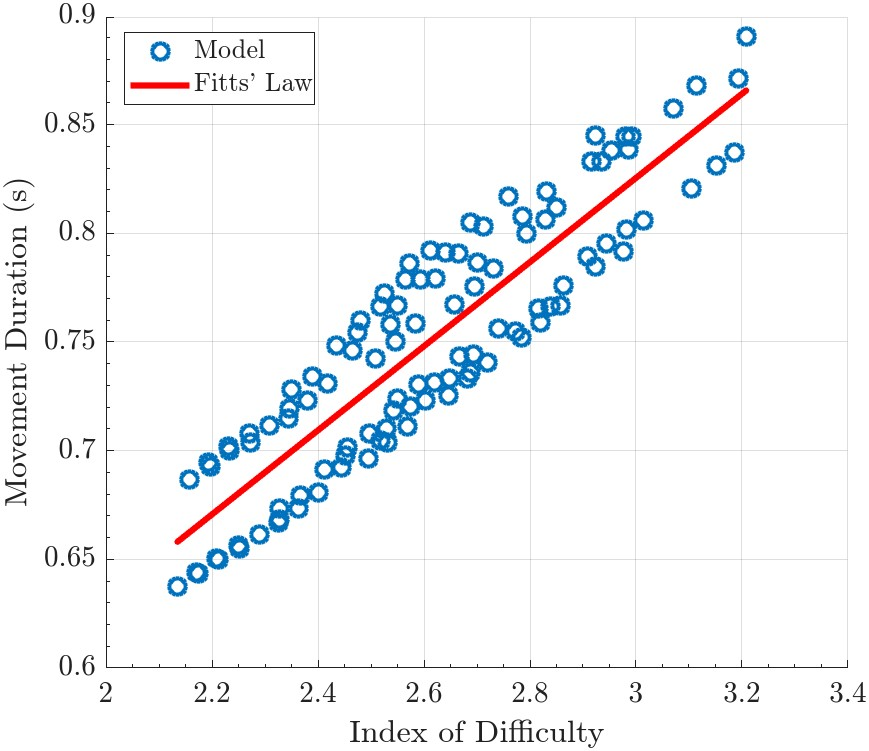
\includegraphics[width=0.8\linewidth]{images/final_fitts_law_single.jpg}
    \caption{Speed-accuracy tradeoff for the feedforward model.}
    \label{fig:FittsLawSingle}
\end{figure}

\begin{figure}[h]
    \centering
    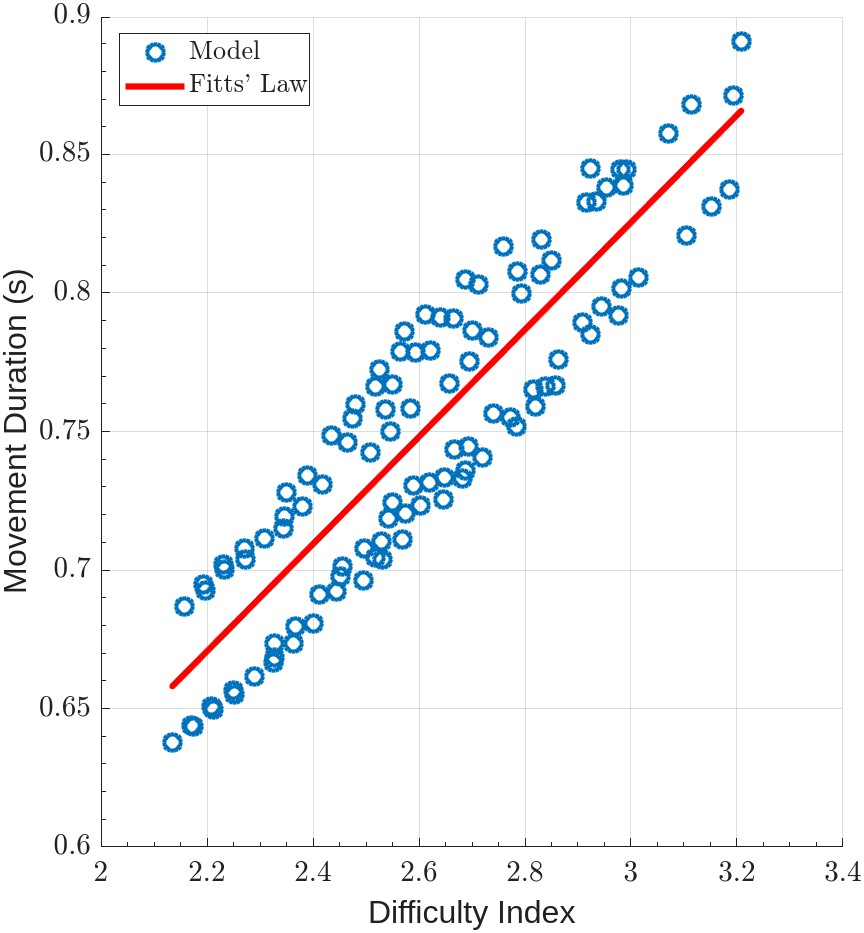
\includegraphics[width=0.8\linewidth]{images/final_fitts_law_mpc.jpg}
    \caption{Speed-accuracy tradeoff for the feedback MPC model.}
    \label{fig:FittsLawMPC}
\end{figure}

Both models produce $a,b$ values that fall within the experimentally observed ranges of $a \in [0.0047, 0.5239]$ and $b \in [0.0393,0.1987]$ reported in \cite{fitts_law_exp_data}, and their $R^2$ values indicate good agreement with Fitts' Law.
\todo{discuss significance of different parameters between models, higher variance data in MPC model}
%  These values are similar to those produced by a motor noise only model with $R^2 = 0.85$ \cite{signal_dependent_motor_noise} and a torque model with $R^2 = 0.88$ \cite{original_paper_high_fidelity}. However, they fall short of the high fidelity model, which produced $R^2 = 0.974$ \cite{original_paper_high_fidelity}.

%  This level of agreement is similar to that produced by a motor noise only model with \(R^2 = 0.85\) \cite{signal_dependent_motor_noise} and a torque model with \(R^2 = 0.88\)\cite{original_paper_high_fidelity}.
%  However, it falls short of the the high fidelity model, which produced \(R^2 = 0.974\)\cite{original_paper_high_fidelity}.
%  We suspect the combination of both motor noise and trajectory optimization on a lower fidelity model can account for the somewhat lower quality of fit compared to the high fidelity model.
%  Another consideration to be made in regards to our model is the challenge of producing high index of difficulty simulations from decreasing the target size. 
%  Due to the uncertainty created by motor noise in our optimization process, the simulation is unable to reliably converge in simulations which use a target radius of less than 0.01m, which limited our capability to create a Fitts' law model solely by changing the size of the target. As a result, we used simulations which varied index of difficulty using both distance to the target and target size. 

Since our models are both able to partially replicate the kinematic profiles of real reaching experiments, and the movement duration predicted by our simulations can be predicted by Fitts' Law, our model is reasonably effective at representing the speed-accuracy tradeoff phenomenon.
Our model surpasses the capabilities of a simple torque model, indicating that trajectory optimization while applying signal dependent motor noise to muscle activation is an effective and promising method for improving the modeling of human reaching.
Both noise and trajectory optimization appear to be valid explanations for speed-accuracy tradeoff, and they are not mutually exclusive.

\begin{figure}[h]
    \centering
    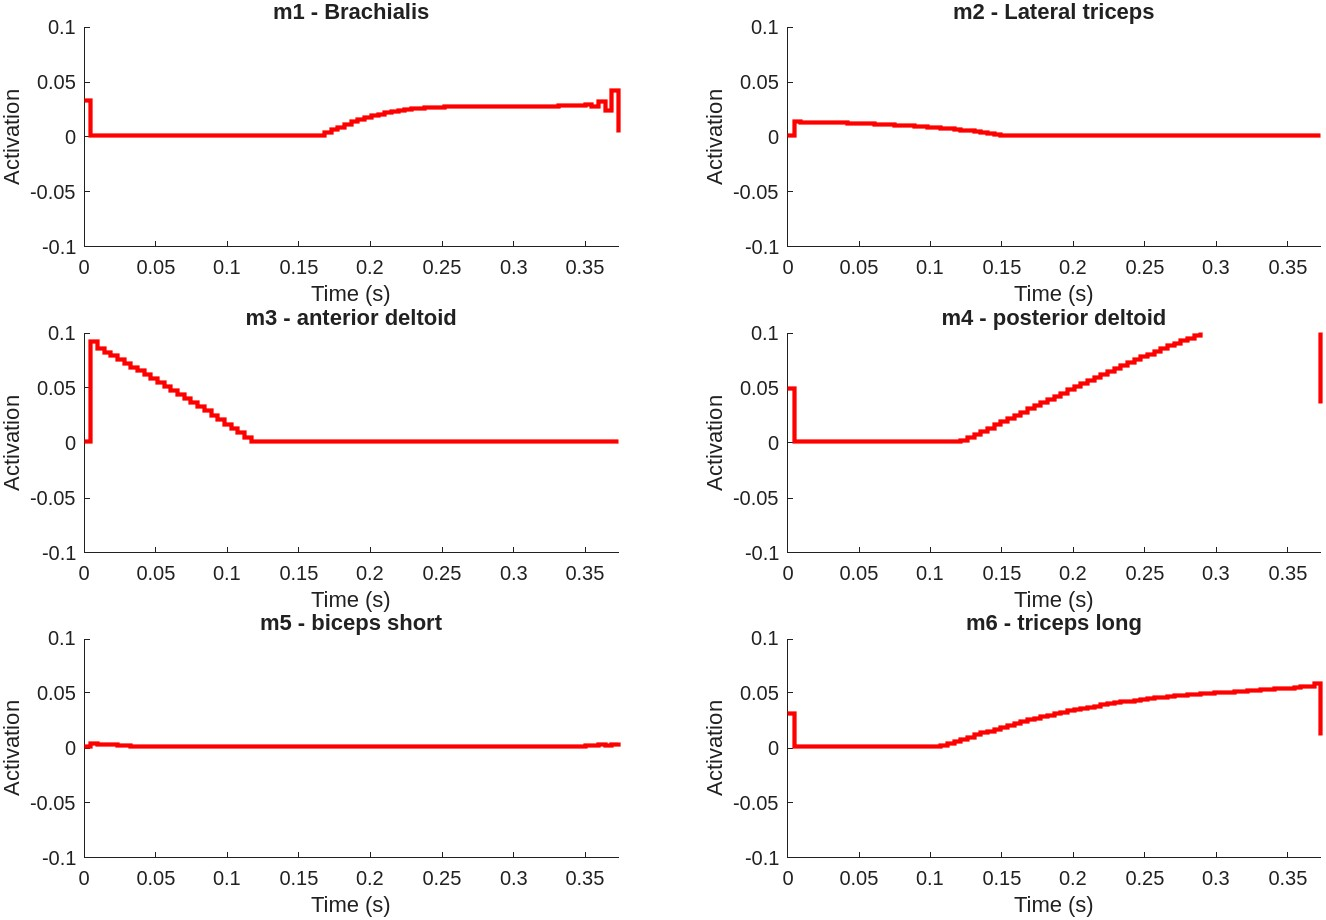
\includegraphics[width=0.45\textwidth]{images/demo_activations_small.jpg}
    \caption{Muscle activation trajectories for a reaching task using the Van Wouwe model.}
    \label{fig:demo_activations}
\end{figure}

\begin{figure}[h]
    \centering
    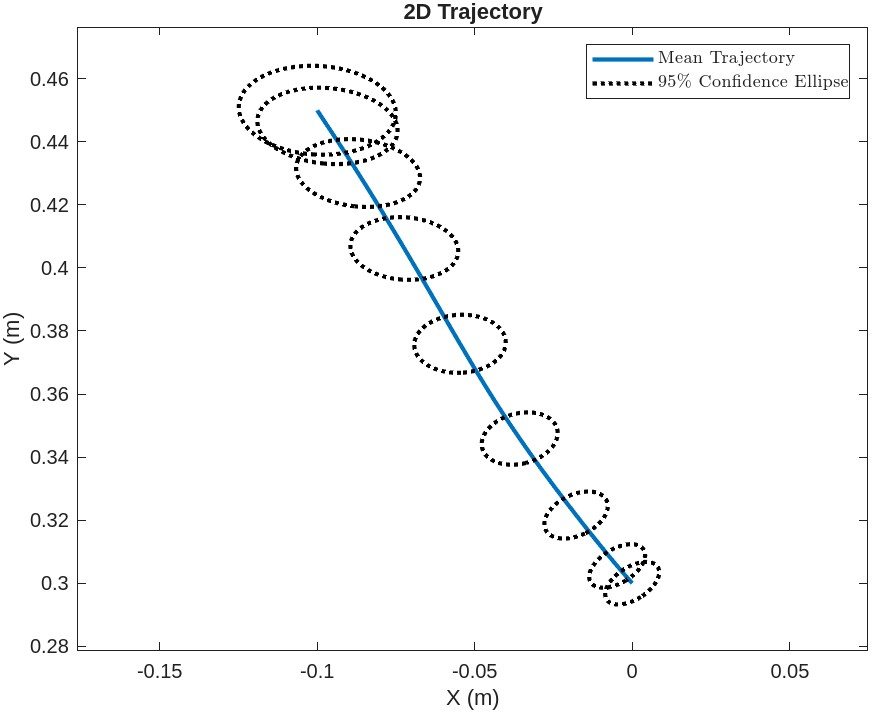
\includegraphics[width=0.45\textwidth]{images/demo_traj_small.jpg}
    \caption{End Effector trajectory for reaching task using the Van Wouwe model.}
    \label{fig:demo_position}
\end{figure}

\section{Limitations and Future Work}
% Overall, the results of our simulations indicate a model utilizing both trajectory optimization and signal dependent motor noise can be used to demonstrate the speed-accuracy tradeoff. 

% One limitation of our work is the inaccuracy of our Gaussian noise model. Due to the highly nonlinear nature of our musculoskeletal arm model caused both by rotating joints and nonlinear muscle actuation, the assumption that the state and end effector distributions remain Gaussian is very inaccurate.
% While this was approximation was sufficient to demonstrate the high level findings, a more accurate noise model may lead to more accurate results with respect to replication of experimental data.
% Additionally, comparison of different noise models could provide information about the noise model used internally by the human brain.
One limitation of this work is the lack of a more complex arm model. While the 2D model was sufficient to demonstrate the speed-accuracy tradeoff, a more complex model like the one used in \cite{original_paper_high_fidelity} could provide more biologically realistic data and results, and would allow us to interpet the details of our simulated results rather than simply looking at high level trends.
% Our simplified 2D model replicates speed-accuracy tradeoff, but doesn't capture all the complexity of the human arm, which leads to some degradation in performance when compared to the capabilities of a high fidelity system. 
% There is definitely potential in combining signal dependent motor noise with a high fidelity musculoskeletal model, which would further improve the realism of simulations of end effector trajectories and movement duration. However, we suspect there would be significant challenge to using such a model based off of the difficulties we encountered obtaining convergence for high precision targets using our simplified approach. 

the use of different trajectory optimization methods would allow us to determine the best method for modeling the speed-accuracy tradeoff, and therefore gain insight into the biological accuracy of each method. This could also give us a more fair comparison to the simulated results in \cite{original_paper_high_fidelity}, since they used a different optimization method which could contribute to the comparison. We suspect that with an ideal noise model and optimization technique, signal dependent noise can be fully implemented into a high fidelity musculoskeletal model to achieve the best lifelike simulations.

\todo{mention use of different optimization methods like shooting, also use of stochastic optimization to better simulate natural variation in human movements, mention difficulty with converging}

\todo{mention adding sensor noise and feedback delay to MPC model}
% An additional trait of velocity profiles with slower movements is a tendency for multiple local minima \cite{soechting_target_size}\cite{tanaka_min_variance}. Our model does not display these traits, while the high fidelity model does. As a result, we conclude the two dimensional muscle activation model we use for our optimization is superior to simple torque models with motor noise, it is not detailed enough to fully match the shape of experimental results as a high fidelity model would. 
% \par Our model is also able to replicate the speed-accuracy tradeoff as modeled by Fitts' Law. Our obtained values for a and b (\(a = 0.0604\) and \(b = 0.0759\)) fall well within the ranges \(a \in [0.0047, 0.5239]\), and \(b \in [0.0393,0.1987]\) \cite{fitts_law_exp_data}. The \(R^2\) value of 0.888 obtained indicates good agreement of our model with Fitts' law. This level of agreement is similar to that produced by a motor noise only model with \(R^2 = 0.85\) \cite{signal_dependent_motor_noise} and a torque model with \(R^2 = 0.88\)\cite{original_paper_high_fidelity}. However, it falls short of the the high fidelity model, which produced \(R^2 = 0.974\)\cite{original_paper_high_fidelity}. We suspect the combination of both motor noise and trajectory optimization on a lower fidelity model can account for the somewhat lower quality of fit compared to the high fidelity model. Another consideration to be made in regards to our model is the challenge of producing high index of difficulty simulations from decreasing the target size. Due to the uncertainty created by motor noise in our optimization process, the simulation is unable to reliably converge in simulations which use a target radius of less than 0.01m, which limited our capability to create a Fitts' law model solely by changing the size of the target. As a result, we used simulations which varied index of difficulty using both distance to the target and target size. 

% \par Since our model is able to partially replicate the kinematic profiles of real reaching experiments, and the movement duration predicted by our simulations can be predicted by Fitts' Law, our model is reasonably effective at representing the speed-accuracy tradeoff phenomenon. Our model surpasses the capabilities of a simple torque model, indicating that trajectory optimization while applying signal dependent motor noise to muscle activation is an effective and promising method for improving the modeling of human reaching. Both noise and trajectory optimization appear to be valid explanations for speed-accuracy tradeoff, and they are not mutually exclusive. Our simplified 2D model replicates speed-accuracy tradeoff, but doesn't capture all the complexity of the human arm, which leads to some degradation in performance when compared to the capabilities of a high fidelity system. There is definitely potential in combining signal dependent motor noise with a high fidelity musculoskeletal model, which would further improve the realism of simulations of end effector trajectories and movement duration. However, we suspect there would be significant challenge to using such a model based off of the difficulties we encountered obtaining convergence for high precision targets using our simplified approach. 

% Overall, we were able to accomplish all of our baseline goals. We successfully developed a model that was able to incorporate signal dependent motor noise into a trajectory optimization problem, and were able to run a sufficient number of experimental trials using this model. Additionally, we were able to make insightful comparisons of our simulated data to data from previous works, including experimental data from human subjects. While we did not have time to explore our reach goals of comparing performance of different trajectory optimization methods, we generally achieved the desired result from this project.

\printbibliography
\end{document}
